\chapter{Setting Up the Project}

\section{Hardware Setup}

\subsection{Equipment List}
\begin{itemize}
	\item A computer that can be mounted on the robot. The computer must run on Linux Ubuntu (13.10 or 14.04 for ROS Indigo) and have a Bluetooth adapter.
	\item Two wireless routers (for example TP-Link).
	\item Two sinus inverters. One power inverter from Biltema and a silver colored pure sine inverter.
	\item One 12V Battery. The battery used in this project has a capacity of $45 Ah$.
	\item A $230V AC/24V DC$ converter.
	\item One XMEGA A3BU evalation board.
	\item One Hokuyo URG-04LX-UG01 LIDAR.
	\item A Kinect for XBOX 360 or an equivalent OpenNI depth camera.
\end{itemize}

\begin{figure}[h]
	\centering
	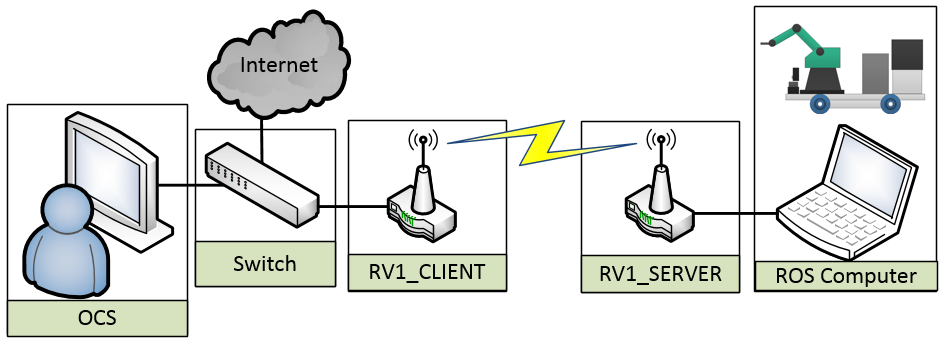
\includegraphics[width=0.85\textwidth]{network_setup}
	\caption{Network hardware setup. }
	\label{fig:network_setup}
\end{figure}

\section{Installation}

\subsection{Software list}

\begin{description}
	\item[Hector SLAM for ROS] Install with \begin{verbatim} sudo apt-get install ros-indigo-hector-slam \end{verbatim}
	\item[Web video server node] Install with \begin{verbatim} sudo apt-get install ros-indigo-web-video-server \end{verbatim}
	\item[LIDAR driver] Install with \begin{verbatim} sudo apt-get install ros-indigo-hokuyo-node \end{verbatim}
\end{description}



\subsubsection{Compatibility Issues}

Indigo, Ubuntu etc.

\subsection{Install Ubuntu}

\subsection{Download ROS}

\section{Configuring the Project}

\subsection{Configuring the ROS Workspace}

\subsection{Configuring the Bluetooth Connection}

The Qt framework is used to simplify the implementation of the Bluetooth connection between the \ac{ROS} graph and a remote device. Our \ac{ROS} installation for this project already includes some variant of Qt version 4.8. While useful for creating new \ac{GUI} applications, it lacks a Bluetooth API. The latest version of Qt, version 5.x, is equipped with libraries necessary for developing Bluetooth applications. This part of the guide will explain how to create a Qt 5 application which can be build by \texttt{catkin\_make} and run as a \textit{rosnode}.

\subsubsection{1 - Install Qt5}

Installing Qt5 for Linux is a straight forward procedure. Go to \url{qt.io}, and download the free version of Qt. All necessary instructions are provided. Qt5 may be installed in the home folder.

\subsubsection{2- Enabling Qt5 in a ROS node}

It is assumed that the \ac{ROS} package \texttt{bluetooth\_server}, is located in a catkin workspace:
\begin{verbatim}
	<NAME OF CATKIN WORKSPACE>/src/bluetooth_server
\end{verbatim}

Inside this folder, open the file ''CMakeLists.txt'' and locate the following:

\begin{verbatim}
set(CMAKE_PREFIX_PATH "/home/vegard/Qt/5.5/gcc_64/lib/cmake/Qt5"
					  "/home/vegard/Qt/5.5/gcc_64/lib/cmake/Qt5Core"
					  "/home/vegard/Qt/5.5/gcc_64/lib/cmake/Qt5Bluetooth"
\end{verbatim}

Change these paths to the correct paths on your system.

% FJERN DETTE DELKAPITTELET!
%\subsection{Adding the Qwt Plugin For Customizing QDial}

%This is a ''howto'' guide on how to install the Qwt-plugin.The following is assumed:

%\begin{itemize}
%	\item Development is performed on Windows 7
%	\item Qt 5.x is installed at c:/Qt
%\end{itemize}

\section{System Launch Procedure}

Preparations:

\begin{enumerate}
	\item Open four terminal windows.	
\end{enumerate}